\documentclass{article}\usepackage[]{graphicx}\usepackage[]{xcolor}
% maxwidth is the original width if it is less than linewidth
% otherwise use linewidth (to make sure the graphics do not exceed the margin)
\makeatletter
\def\maxwidth{ %
  \ifdim\Gin@nat@width>\linewidth
    \linewidth
  \else
    \Gin@nat@width
  \fi
}
\makeatother

\definecolor{fgcolor}{rgb}{0.345, 0.345, 0.345}
\newcommand{\hlnum}[1]{\textcolor[rgb]{0.686,0.059,0.569}{#1}}%
\newcommand{\hlsng}[1]{\textcolor[rgb]{0.192,0.494,0.8}{#1}}%
\newcommand{\hlcom}[1]{\textcolor[rgb]{0.678,0.584,0.686}{\textit{#1}}}%
\newcommand{\hlopt}[1]{\textcolor[rgb]{0,0,0}{#1}}%
\newcommand{\hldef}[1]{\textcolor[rgb]{0.345,0.345,0.345}{#1}}%
\newcommand{\hlkwa}[1]{\textcolor[rgb]{0.161,0.373,0.58}{\textbf{#1}}}%
\newcommand{\hlkwb}[1]{\textcolor[rgb]{0.69,0.353,0.396}{#1}}%
\newcommand{\hlkwc}[1]{\textcolor[rgb]{0.333,0.667,0.333}{#1}}%
\newcommand{\hlkwd}[1]{\textcolor[rgb]{0.737,0.353,0.396}{\textbf{#1}}}%
\let\hlipl\hlkwb

\usepackage{framed}
\makeatletter
\newenvironment{kframe}{%
 \def\at@end@of@kframe{}%
 \ifinner\ifhmode%
  \def\at@end@of@kframe{\end{minipage}}%
  \begin{minipage}{\columnwidth}%
 \fi\fi%
 \def\FrameCommand##1{\hskip\@totalleftmargin \hskip-\fboxsep
 \colorbox{shadecolor}{##1}\hskip-\fboxsep
     % There is no \\@totalrightmargin, so:
     \hskip-\linewidth \hskip-\@totalleftmargin \hskip\columnwidth}%
 \MakeFramed {\advance\hsize-\width
   \@totalleftmargin\z@ \linewidth\hsize
   \@setminipage}}%
 {\par\unskip\endMakeFramed%
 \at@end@of@kframe}
\makeatother

\definecolor{shadecolor}{rgb}{.97, .97, .97}
\definecolor{messagecolor}{rgb}{0, 0, 0}
\definecolor{warningcolor}{rgb}{1, 0, 1}
\definecolor{errorcolor}{rgb}{1, 0, 0}
\newenvironment{knitrout}{}{} % an empty environment to be redefined in TeX

\usepackage{alltt}
\usepackage[margin=1.0in]{geometry} % To set margins
\usepackage{amsmath}  % This allows me to use the align functionality.
                      % If you find yourself trying to replicate
                      % something you found online, ensure you're
                      % loading the necessary packages!
\usepackage{amsfonts} % Math font
\usepackage{fancyvrb}
\usepackage{hyperref} % For including hyperlinks
\usepackage[shortlabels]{enumitem}% For enumerated lists with labels specified
                                  % We had to run tlmgr_install("enumitem") in R
\usepackage{float}    % For telling R where to put a table/figure
\usepackage{natbib}        %For the bibliography
\bibliographystyle{apalike}%For the bibliography
\IfFileExists{upquote.sty}{\usepackage{upquote}}{}
\begin{document}

In lecture 16, we looked at precipitation amounts in Madison County (at 
Morrisville station). We found that the Weibull distribution had a good fit
to the monthly precipitation amounts.\\

We found that the MLEs for the Weibull distribution were 
\begin{align*}
    \hat{a}&=2.1871\\
    \hat{\sigma}&=3.9683
\end{align*}
and
\[-\mathcal{L}(\{\hat{a}, \hat{\sigma}\}|\mathbf{x}) = 2166.496\]
is the realized negative log-likelihood.
Note this means that the log-likelihood is
\[\mathcal{L}(\{\hat{a}, \hat{\sigma}\}|\mathbf{x}) = -2166.496,\]
and the usual likelihood is
\[L(\{\hat{a}, \hat{\sigma}\}|\mathbf{x}) = e^{\left[\mathcal{L}(\{\hat{a}, \hat{\sigma}\}|\mathbf{x})\right]} \approx = e^{-2166.496},\]
which \texttt{R} cannot differentiate from 0.

\begin{enumerate}
  \item Someone asked ``why Weibull?" in class. That is, why wouldn't we use 
  another right-skewed distribution like the Gamma (see Lecture 15), or
  the Log-Normal (see Lecture 17).
  \begin{enumerate}
    \item Compute the MLEs for these data using a Gamma distribution.\\ 
    \texttt{Solution:} The MLEs for these data using a Gamma distribution are
    \begin{align*}
      \hat{a}&=4.17\\
      \hat{\beta}&=1.19 
    \end{align*}
    \[\mathcal{L}(\{\hat{a}, \hat{\beta}\}|\mathbf{x}) = -2151.149\]
    \item Compute the MLEs for these data using the Log-Normal distribution. \\
    \texttt{Solution:} The MLEs for these data using a Log-Normal distribution are
    \begin{align*}
      \hat{\mu}&=1.131\\
      \hat{\sigma}&=0.533 
    \end{align*}
    \[\mathcal{L}(\{\hat{\mu}, \hat{\sigma}\}|\mathbf{x}) = -2204.201\]
    \item Compute the likelihood ratio to compare the Weibull and the Gamma distribution. 
    Which has a better fit according to the likelhiood ratio?
    \[Q = \frac{L(\{\hat{a}, \hat{\sigma}\}|\mathbf{x})}{L(\{\hat{\alpha}, \hat{\beta}\}|\mathbf{x})}=e^{\left[\mathcal{L}(\{\hat{a}, \hat{\sigma}\}|\mathbf{x}) - \mathcal{L}(\{\hat{\alpha}, \hat{\beta}\}|\mathbf{x})\right]}\]
    \texttt{Solution:} According to the likelihood ratio, the Weibull distribution has a better
    fit since the ratio has a value $>$ 1, suggesting the top model (Weibull) as the better fit.
    \\
    \item Compute the likelihood ratio to compare the Weibull and the Log-Normal distribution.
    Which has a better fit according to the likelihood ratio? 
    \[Q = \frac{L(\{\hat{a}, \hat{\sigma}\}|\mathbf{x})}{L(\{\hat{\mu}, \hat{\sigma}\}|\mathbf{x})}=e^{\left[\mathcal{L}(\{\hat{a}, \hat{\sigma}\}|\mathbf{x}) - \mathcal{L}(\{\hat{\mu}, \hat{\sigma}\}|\mathbf{x})\right]}\]
    \texttt{Solution:} According to the likelihood ratio, the Log-Normal distribution has a         better fit since the ratio has a value $<$ 1, suggesting the bottom model (Log-Normal) as       the better fit.
    \\
    \item Compute the likelihood ratio to compare the Gamma and the Log-Normal distribution.
    Which has a better fit according to the likelhiood ratio?
    \[Q = \frac{L(\{\hat{\alpha}, \hat{\beta}\}|\mathbf{x})}{L(\{\hat{\mu}, \hat{\sigma}\}|\mathbf{x})}=e^{\left[\mathcal{L}(\{\hat{\alpha}, \hat{\beta}\}|\mathbf{x}) - \mathcal{L}(\{\hat{\mu}, \hat{\sigma}\}|\mathbf{x})\right]}\]
    \texttt{Solution:} According to the likelihood ratio, the Log-Normal distribution has a         better fit since the ratio has a value $<$ 1, suggesting the bottom model (Log-Normal) as       the better fit
  \end{enumerate}
  
\texttt{Code for Question 1:}
\begin{knitrout}\scriptsize
\definecolor{shadecolor}{rgb}{0.969, 0.969, 0.969}\color{fgcolor}\begin{kframe}
\begin{alltt}
\hldef{rain.data} \hlkwb{=} \hlkwd{read_csv}\hldef{(}\hlsng{"agacis.csv"}\hldef{)} \hlcom{#Load the data set}
\end{alltt}


{\ttfamily\noindent\itshape\color{messagecolor}{\#\# Rows: 115 Columns: 14\\\#\# -- Column specification --------------------------------------------------------\\\#\# Delimiter: "{},"{}\\\#\# chr (13): Jan, Feb, Mar, Apr, May, Jun, Jul, Aug, Sep, Oct, Nov, Dec, Annual\\\#\# dbl \ (1): Year\\\#\# \\\#\# i Use `spec()` to retrieve the full column specification for this data.\\\#\# i Specify the column types or set `show\_col\_types = FALSE` to quiet this message.}}\begin{alltt}
\hldef{rain.data} \hlkwb{<-} \hldef{rain.data |>}
  \hlkwd{select}\hldef{(}\hlopt{-}\hldef{Annual) |>}                          \hlcom{# Remove annual column }
  \hlkwd{pivot_longer}\hldef{(}\hlkwc{cols} \hldef{=} \hlkwd{c}\hldef{(Jan, Feb, Mar, Apr,}   \hlcom{# pivot the column data into one col}
                        \hldef{May, Jun, Jul, Aug,}
                        \hldef{Sep, Oct, Nov, Dec),}
               \hlkwc{values_to} \hldef{=} \hlsng{"Precipitation"}\hldef{,}   \hlcom{# store the values in Precipitation}
               \hlkwc{names_to} \hldef{=} \hlsng{"Month"}\hldef{) |>}         \hlcom{# store the months in Month}
  \hlkwd{mutate}\hldef{(}\hlkwc{Precipitation} \hldef{=} \hlkwd{case_when}\hldef{(Precipitation} \hlopt{==} \hlsng{"M"} \hlopt{~} \hlnum{NA_character_}\hldef{,}
                                   \hlnum{TRUE}                 \hlopt{~} \hldef{Precipitation))|>}
  \hlkwd{mutate}\hldef{(}\hlkwc{Precipitation} \hldef{=} \hlkwd{as.numeric}\hldef{(Precipitation))}

\hldef{MLE.Weibull} \hlkwb{<-} \hlkwa{function}\hldef{(}\hlkwc{par}\hldef{,}    \hlcom{#parameters arguement}
                        \hlkwc{data}\hldef{,}   \hlcom{#dataframe arguement}
                        \hlkwc{neg}\hldef{=F)\{} \hlcom{#negative arguement}
  \hlcom{#FUNCTION PURPOSE:}
  \hlcom{#Use Maximum Log Likelihood to estimate parameters for a Weibull distribution for}
  \hlcom{#a given data set}
  \hldef{a} \hlkwb{<-} \hldef{par[}\hlnum{1}\hldef{]}     \hlcom{#Alpha parameter}
  \hldef{sigma} \hlkwb{<-} \hldef{par[}\hlnum{2}\hldef{]} \hlcom{#Sigma parameter}

  \hlcom{#Calculate the log likelihood for given parameters}
  \hldef{ll.like} \hlkwb{<-} \hlkwd{sum}\hldef{(}\hlkwd{log}\hldef{(}\hlkwd{dweibull}\hldef{(}\hlkwc{x} \hldef{= data,} \hlkwc{shape} \hldef{= a,} \hlkwc{scale} \hldef{= sigma)),} \hlkwc{na.rm}\hldef{=T)}

  \hlkwd{return}\hldef{(}\hlkwd{ifelse}\hldef{(neg,} \hlopt{-}\hldef{ll.like, ll.like))} \hlcom{#If neg is True, return the result as a negative}
\hldef{\}}

\hldef{MLE.Weibull.data} \hlkwb{<-} \hlkwd{optim}\hldef{(}\hlkwc{fn} \hldef{= MLE.Weibull,} \hlcom{#Using optim, estimate the parameters }
                          \hlkwc{par} \hldef{=} \hlkwd{c}\hldef{(}\hlnum{1}\hldef{,}\hlnum{1}\hldef{),}     \hlcom{#at which the log likelihood is at it's min}
                          \hlkwc{data} \hldef{= rain.data}\hlopt{$}\hldef{Precipitation,}
                          \hlkwc{neg}\hldef{=T)}            \hlcom{#(i.e. finds the parameters for the data's distribution)}

\hldef{MLE.Gamma} \hlkwb{<-} \hlkwa{function}\hldef{(}\hlkwc{data}\hldef{,}          \hlcom{#dataframe argument}
                      \hlkwc{para}\hldef{,}          \hlcom{#parameters argument}
                      \hlkwc{neg} \hldef{=} \hlnum{FALSE}\hldef{) \{} \hlcom{#negative argument}
  \hlcom{#FUNCTION PURPOSE:}
  \hlcom{#Use Maximum Log Likelihood to estimate parameters for a Gamma distribution for}
  \hlcom{#a given data set}
  \hldef{alpha} \hlkwb{<-} \hldef{para[}\hlnum{1}\hldef{]} \hlcom{#Alpha parameter}
  \hldef{beta} \hlkwb{<-} \hldef{para[}\hlnum{2}\hldef{]}  \hlcom{#Beta parameter}

  \hlcom{#Calculate the log likelihood for given parameters}
  \hldef{ll.like} \hlkwb{<-} \hlkwd{sum}\hldef{(}\hlkwd{log}\hldef{(}\hlkwd{dgamma}\hldef{(data,} \hlkwc{shape} \hldef{= alpha,} \hlkwc{rate} \hldef{= beta)),} \hlkwc{na.rm} \hldef{=} \hlnum{TRUE}\hldef{)}

  \hlkwd{return}\hldef{(}\hlkwd{ifelse}\hldef{(neg,} \hlopt{-}\hldef{ll.like, ll.like))} \hlcom{#If neg is True, return the result as a negative}
\hldef{\}}

\hldef{MLE.Gamma.data} \hlkwb{<-} \hlkwd{optim}\hldef{(}\hlkwc{fn} \hldef{= MLE.Gamma,} \hlcom{#Using optim, estimate the parameters}
                        \hlkwc{par} \hldef{=} \hlkwd{c}\hldef{(}\hlnum{1}\hldef{,}\hlnum{1}\hldef{),}   \hlcom{#at which the log likelihood is at it's min}
                        \hlkwc{data} \hldef{= rain.data}\hlopt{$}\hldef{Precipitation,}
                        \hlkwc{neg} \hldef{=} \hlnum{TRUE}\hldef{)}     \hlcom{#(i.e. finds the parameters for the data's distribution)}

\hldef{MLE.LogNorm} \hlkwb{<-} \hlkwa{function}\hldef{(}\hlkwc{data}\hldef{,}          \hlcom{#dataframe argument}
                        \hlkwc{para}\hldef{,}          \hlcom{#parameters argument}
                        \hlkwc{neg} \hldef{=} \hlnum{FALSE}\hldef{) \{} \hlcom{#negative argument}
  \hlcom{#FUNCTION PURPOSE:}
  \hlcom{#Use Maximum Log Likelihood to estimate parameters for a Log Normal distribution for}
  \hlcom{#a given data set}
  \hldef{mu} \hlkwb{<-} \hldef{para[}\hlnum{1}\hldef{]}     \hlcom{#Mu parameter}
  \hldef{sigma} \hlkwb{<-} \hldef{para[}\hlnum{2}\hldef{]}  \hlcom{#Sigma parameter}

  \hlcom{#Calculate the log likelihood for given parameters}
  \hldef{ll.like} \hlkwb{<-} \hlkwd{sum}\hldef{(}\hlkwd{log}\hldef{(}\hlkwd{dlnorm}\hldef{(data,} \hlkwc{meanlog} \hldef{= mu,} \hlkwc{sdlog} \hldef{= sigma)),} \hlkwc{na.rm} \hldef{=} \hlnum{TRUE}\hldef{)}

  \hlkwd{return}\hldef{(}\hlkwd{ifelse}\hldef{(neg,} \hlopt{-}\hldef{ll.like, ll.like))} \hlcom{#If neg is True, return the result as a negative}
\hldef{\}}

\hldef{MLE.LogNorm.data} \hlkwb{<-} \hlkwd{optim}\hldef{(}\hlkwc{fn} \hldef{= MLE.LogNorm,}  \hlcom{#Using optim, estimate the parameters}
                          \hlkwc{par} \hldef{=} \hlkwd{c}\hldef{(}\hlnum{1}\hldef{,}\hlnum{1}\hldef{),}      \hlcom{#at which the log likelihood is at it's min}
                          \hlkwc{data} \hldef{= rain.data}\hlopt{$}\hldef{Precipitation,}
                          \hlkwc{neg} \hldef{=} \hlnum{TRUE}\hldef{)}        \hlcom{#(i.e. finds the parameters for the data's distribution)}

\hldef{LR1} \hlkwb{<-} \hldef{MLE.Weibull.data}\hlopt{$}\hldef{value}\hlopt{/}\hldef{MLE.Gamma.data}\hlopt{$}\hldef{value}   \hlcom{#Calculates the Likelihood ratio for Weibull and Gamma distribution}
\hldef{LR2} \hlkwb{<-} \hldef{MLE.Weibull.data}\hlopt{$}\hldef{value}\hlopt{/}\hldef{MLE.LogNorm.data}\hlopt{$}\hldef{value} \hlcom{#Calculates the Likelihood ratio for Weibull and Log Normal distribution}
\hldef{LR3} \hlkwb{<-} \hldef{MLE.Gamma.data}\hlopt{$}\hldef{value}\hlopt{/}\hldef{MLE.LogNorm.data}\hlopt{$}\hldef{value}   \hlcom{#Calculates the Likelihood ratio for Gamma and Log Normal distribution}
\end{alltt}
\end{kframe}
\end{knitrout}
  
  \item Optional Coding Challenge. Choose the ``best" distribution and refit the
  model by season.
  \begin{enumerate}
    \item Fit the Distribution for Winter (December-February).\\
    \texttt{Solution:} The best fit distribution for Winter is a Weibull distribution.
    \item Fit the Distribution for Spring (March-May).\\
    \texttt{Solution:} The best fit distribution for Spring is a Lognormal distribution.
    \item Fit the Distribution for Summer (June-August).\\
    \texttt{Solution:} The best fit distribution for Summer is a Lognormal distribution.
    \item Fit the Distribution for Fall (September-November).\\
    \texttt{Solution:} The best fit distribution for Fall is a Lognormal distribution.
    \item Plot the four distributions in one plot using \texttt{cyan3} for Winter,
    \texttt{chartreuse3} for Spring, \texttt{red3} for Summer, and \texttt{chocolate3}
    for Fall. Note any similarities/differences you observe across the seasons.
  \end{enumerate}
\end{enumerate}

\texttt{Code for Question 2:}
\begin{knitrout}\scriptsize
\definecolor{shadecolor}{rgb}{0.969, 0.969, 0.969}\color{fgcolor}\begin{kframe}
\begin{alltt}
\hldef{winter.data} \hlkwb{<-} \hldef{rain.data |>}
  \hlkwd{filter}\hldef{(Month} \hlopt \hlkwd{c}\hldef{(}\hlsng{"Dec"}\hldef{,} \hlsng{"Jan"}\hldef{,} \hlsng{"Feb"}\hldef{))} \hlcom{#Filter only the winter months}

\hldef{spring.data} \hlkwb{<-} \hldef{rain.data |>}
  \hlkwd{filter}\hldef{(Month} \hlopt \hlkwd{c}\hldef{(}\hlsng{"Mar"}\hldef{,} \hlsng{"Apr"}\hldef{,} \hlsng{"May"}\hldef{))} \hlcom{#Filter only the spring moneths}

\hldef{summer.data} \hlkwb{<-} \hldef{rain.data |>}
  \hlkwd{filter}\hldef{(Month} \hlopt \hlkwd{c}\hldef{(}\hlsng{"Jun"}\hldef{,} \hlsng{"Jul"}\hldef{,} \hlsng{"Aug"}\hldef{))} \hlcom{#Filter only the summer months}

\hldef{fall.data} \hlkwb{<-} \hldef{rain.data |>}
  \hlkwd{filter}\hldef{(Month} \hlopt \hlkwd{c}\hldef{(}\hlsng{"Sep"}\hldef{,} \hlsng{"Oct"}\hldef{,} \hlsng{"Nov"}\hldef{))} \hlcom{#Filter only the fall months}

\hldef{data.list} \hlkwb{<-} \hlkwd{list}\hldef{(}\hlkwc{winter} \hldef{= winter.data,} \hlcom{#Place all the filtered data sets into a list}
                  \hlkwc{spring} \hldef{= spring.data,}
                  \hlkwc{summer} \hldef{= summer.data,}
                  \hlkwc{fall} \hldef{= fall.data)}
\hldef{best.fit.results} \hlkwb{=} \hlkwd{c}\hldef{()} \hlcom{#Will store the best distribution for each season}

\hlkwa{for}\hldef{(data} \hlkwa{in} \hldef{data.list) \{} \hlcom{#For each season}
  \hldef{MLE.Weibull.data} \hlkwb{<-} \hlkwd{optim}\hldef{(}\hlkwc{fn} \hldef{= MLE.Weibull,} \hlcom{#Gather the Log Likelihood estimate }
                            \hlkwc{par} \hldef{=} \hlkwd{c}\hldef{(}\hlnum{1}\hldef{,}\hlnum{1}\hldef{),}     \hlcom{#using optim}
                            \hlkwc{data} \hldef{= data}\hlopt{$}\hldef{Precipitation,}
                            \hlkwc{neg}\hldef{=T)}
  \hldef{MLE.Gamma.data} \hlkwb{<-} \hlkwd{optim}\hldef{(}\hlkwc{fn} \hldef{= MLE.Gamma,}     \hlcom{#Gather the Log Likelihood estimate}
                          \hlkwc{par} \hldef{=} \hlkwd{c}\hldef{(}\hlnum{1}\hldef{,}\hlnum{1}\hldef{),}       \hlcom{#using optim}
                          \hlkwc{data} \hldef{= data}\hlopt{$}\hldef{Precipitation,}
                          \hlkwc{neg} \hldef{=} \hlnum{TRUE}\hldef{)}
  \hldef{MLE.LogNorm.data} \hlkwb{<-} \hlkwd{optim}\hldef{(}\hlkwc{fn} \hldef{= MLE.LogNorm,} \hlcom{#Gather the Log Likelihood estimate}
                            \hlkwc{par} \hldef{=} \hlkwd{c}\hldef{(}\hlnum{1}\hldef{,}\hlnum{1}\hldef{),}     \hlcom{#using optim}
                            \hlkwc{data} \hldef{= data}\hlopt{$}\hldef{Precipitation,}
                            \hlkwc{neg} \hldef{=} \hlnum{TRUE}\hldef{)}

  \hldef{LR1} \hlkwb{<-} \hldef{MLE.Weibull.data}\hlopt{$}\hldef{value}\hlopt{/}\hldef{MLE.Gamma.data}\hlopt{$}\hldef{value}   \hlcom{#Calculates the Likelihood ratio for Weibull and Gamma distribution}
  \hldef{LR2} \hlkwb{<-} \hldef{MLE.Weibull.data}\hlopt{$}\hldef{value}\hlopt{/}\hldef{MLE.LogNorm.data}\hlopt{$}\hldef{value} \hlcom{#Calculates the Likelihood ratio for Weibull and Log Normal distribution}
  \hldef{LR3} \hlkwb{<-} \hldef{MLE.Gamma.data}\hlopt{$}\hldef{value}\hlopt{/}\hldef{MLE.LogNorm.data}\hlopt{$}\hldef{value}   \hlcom{#Calculates the Likelihood ratio for Gamma and Log Normal distribution}

  \hlkwa{if}\hldef{(LR1} \hlopt{>} \hlnum{1} \hlopt{&&} \hldef{LR2} \hlopt{>} \hlnum{1}\hldef{)\{} \hlcom{#If Weibull is favored between the Gamma and Log Normal}
    \hldef{best.fit} \hlkwb{<-} \hlsng{"Weibull"} \hlcom{#Assign best fit to Weibull}
  \hldef{\}} \hlkwa{else if}\hldef{(LR1} \hlopt{<} \hlnum{1} \hlopt{&&} \hldef{LR3} \hlopt{>} \hlnum{1}\hldef{)\{} \hlcom{#If Gamma is favored between the Weibull and Log Normal}
    \hldef{best.fit} \hlkwb{<-} \hlsng{"Gamma"}          \hlcom{#Assign best fit to Gamma}
  \hldef{\}} \hlkwa{else if}\hldef{(LR2} \hlopt{<} \hlnum{1} \hlopt{&&} \hldef{LR3} \hlopt{<} \hlnum{1}\hldef{) \{} \hlcom{#If Log Normal is favored between Weibull and Gamma}
    \hldef{best.fit} \hlkwb{<-} \hlsng{"Log Normal"}      \hlcom{#Assign best fit to Log Normal}
  \hldef{\}} \hlkwa{else} \hldef{\{}
    \hldef{best.fit} \hlkwb{<-} \hlsng{"Tie"} \hlcom{#If there are two distributions with equal fits, assign best fit to be a tie}
  \hldef{\}}

  \hldef{best.fit.results} \hlkwb{<-} \hlkwd{c}\hldef{(best.fit.results, best.fit)} \hlcom{#Store the best fit distributin for each season}
\hldef{\}}

\hldef{winter.plot.data} \hlkwb{<-} \hlkwd{tibble}\hldef{(}\hlkwc{x} \hldef{=} \hlkwd{seq}\hldef{(}\hlnum{0}\hldef{,} \hlnum{30}\hldef{,} \hlkwc{length.out} \hldef{=} \hlnum{1000}\hldef{))} \hlopt \hlcom{#Obtains data points to plot}
  \hlkwd{mutate}\hldef{(}\hlkwc{pdf} \hldef{=} \hlkwd{dweibull}\hldef{(x,} \hlkwc{shape} \hldef{=} \hlnum{2.47}\hldef{,} \hlkwc{scale} \hldef{=} \hlnum{3.35}\hldef{))}           \hlcom{#Winter data distribution}

\hldef{spring.plot.data} \hlkwb{<-} \hlkwd{tibble}\hldef{(}\hlkwc{x} \hldef{=} \hlkwd{seq}\hldef{(}\hlnum{0}\hldef{,} \hlnum{30}\hldef{,} \hlkwc{length.out} \hldef{=} \hlnum{1000}\hldef{))} \hlopt \hlcom{#Obtains data points to plot}
  \hlkwd{mutate}\hldef{(}\hlkwc{pdf} \hldef{=} \hlkwd{dlnorm}\hldef{(}\hlkwc{x} \hldef{= x,} \hlkwc{meanlog} \hldef{=} \hlnum{1.135}\hldef{,} \hlkwc{sdlog} \hldef{=} \hlnum{0.487}\hldef{))}     \hlcom{#Spring data distribution}

\hldef{summer.plot.data} \hlkwb{<-} \hlkwd{tibble}\hldef{(}\hlkwc{x} \hldef{=} \hlkwd{seq}\hldef{(}\hlnum{0}\hldef{,} \hlnum{30}\hldef{,} \hlkwc{length.out} \hldef{=} \hlnum{1000}\hldef{))} \hlopt \hlcom{#Obtains data points to plot}
  \hlkwd{mutate}\hldef{(}\hlkwc{pdf} \hldef{=} \hlkwd{dlnorm}\hldef{(}\hlkwc{x} \hldef{= x,} \hlkwc{meanlog} \hldef{=} \hlnum{1.126}\hldef{,} \hlkwc{sdlog} \hldef{=} \hlnum{0.518}\hldef{))}     \hlcom{#Summer data distribution}

\hldef{fall.plot.data} \hlkwb{<-} \hlkwd{tibble}\hldef{(}\hlkwc{x} \hldef{=} \hlkwd{seq}\hldef{(}\hlnum{0}\hldef{,} \hlnum{30}\hldef{,} \hlkwc{length.out} \hldef{=} \hlnum{1000}\hldef{))} \hlopt   \hlcom{#Obtains data points to plot}
  \hlkwd{mutate}\hldef{(}\hlkwc{pdf} \hldef{=} \hlkwd{dlnorm}\hldef{(}\hlkwc{x} \hldef{= x,} \hlkwc{meanlog} \hldef{=} \hlnum{1.130}\hldef{,} \hlkwc{sdlog} \hldef{=} \hlnum{0.619}\hldef{))}     \hlcom{#Fall data distribution}

\hlkwd{ggplot}\hldef{()} \hlopt{+}
  \hlkwd{geom_line}\hldef{(}\hlkwc{data} \hldef{= winter.plot.data,} \hlkwd{aes}\hldef{(}\hlkwc{x} \hldef{= x,} \hlkwc{y} \hldef{= pdf),} \hlkwc{color} \hldef{=} \hlsng{"cyan3"}\hldef{)} \hlopt{+} \hlcom{#draws winter distribution}
  \hlkwd{geom_line}\hldef{(}\hlkwc{data} \hldef{= spring.plot.data,} \hlkwd{aes}\hldef{(}\hlkwc{x} \hldef{= x,} \hlkwc{y} \hldef{= pdf),} \hlkwc{color} \hldef{=} \hlsng{"chartreuse3"}\hldef{)} \hlopt{+} \hlcom{#draws spring distribution curve}
  \hlkwd{geom_line}\hldef{(}\hlkwc{data} \hldef{= summer.plot.data,} \hlkwd{aes}\hldef{(}\hlkwc{x} \hldef{= x,} \hlkwc{y} \hldef{= pdf),} \hlkwc{color} \hldef{=} \hlsng{"red3"}\hldef{)} \hlopt{+} \hlcom{#draws summer distribution curve}
  \hlkwd{geom_line}\hldef{(}\hlkwc{data} \hldef{= fall.plot.data,} \hlkwd{aes}\hldef{(}\hlkwc{x} \hldef{= x,} \hlkwc{y} \hldef{= pdf),} \hlkwc{color} \hldef{=} \hlsng{"chocolate3"}\hldef{)} \hlcom{#draws fall distribution curve}
\end{alltt}
\end{kframe}
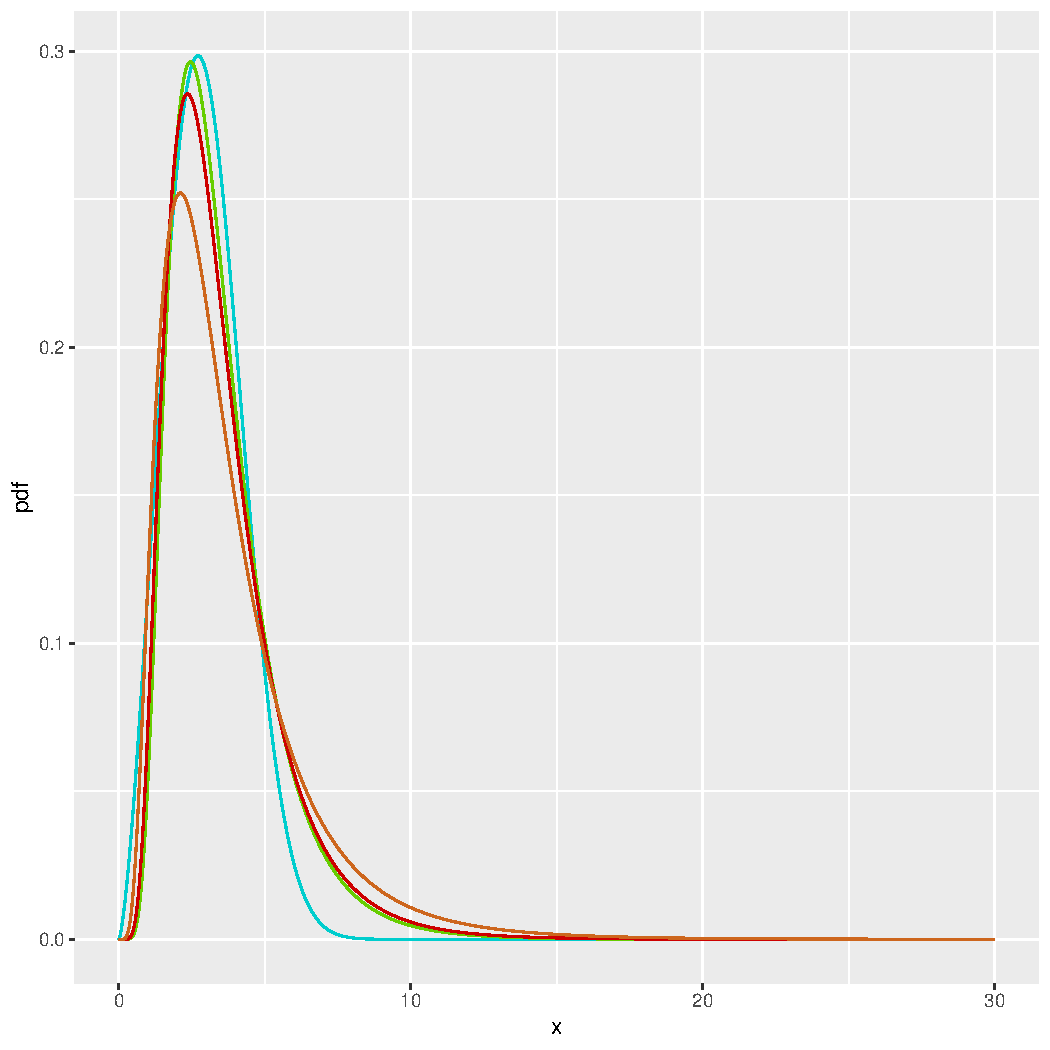
\includegraphics[width=\maxwidth]{figure/unnamed-chunk-3-1} 
\end{knitrout}


\bibliography{bibliography}
\end{document}
